\documentclass[landscape]{article}
\usepackage{graphicx}
\usepackage{fancyhdr}
\usepackage{geometry}
\usepackage[hidelinks]{hyperref}
\usepackage{enumitem}
\usepackage{indentfirst}
\usepackage{titlesec}

\titleformat{\section}{\Large\bfseries}{\thesection}{1em}{}
\titlespacing*{\section}{0pt}{20pt}{10pt}

\newcommand{\machineShortName}{TOM-ICV-66}
\newcommand{\machineName}{IMPRESSORA CORTE E VINCO}
\newcommand{\variant}{2800}
\newcommand{\productionCapacityminimumSheet}{150}
\newcommand{\productionCapacitymaximumSheet}{150}
\newcommand{\minimumSheet}{600x400}
\newcommand{\maximumSheet}{2800x1676,4}
\newcommand{\numberOfPrinters}{5}


% alterar apenas se souber oque o comando ding faz
\newcommand{\dingNumber}{213}

\newif\ifmachineType
%\machineTypetrue % set the variable to true   - FLEXO
\machineTypefalse % set the variable to true - ICV

\newif\ifunidadePerfuradora
\unidadePerfuradoratrue % set the variable to true   - Com perfuradora
%\unidadePerfuradorafalse % set the variable to true - Sem perfuradora

% ######################################
% ########### Flexo WestRock ###########
% ######################################

%\newcommand{\machineShortName}{TOM-IPSDC}
%\newcommand{\machineName}{IMPRESSORA FLEXO FOLDER GLUER}
%\newcommand{\variant}{2600}
%\newcommand{\productionCapacityminimumSheet}{250}
%\newcommand{\productionCapacitymaximumSheet}{70}
%\newcommand{\minimumSheet}{600x300 \space}
%\newcommand{\maximumSheet}{2600x1150 \space}
%\newcommand{\numberOfPrinters}{3}

% ######################################
% ########### ICV WestRock #############
% ######################################

%\newcommand{\machineShortName}{TOM-ICV-66}
%\newcommand{\machineName}{IMPRESSORA CORTE E VINCO}
%\newcommand{\variant}{2800}
%\newcommand{\productionCapacityminimumSheet}{150}
%\newcommand{\productionCapacitymaximumSheet}{150}
%\newcommand{\minimumSheet}{600x400}
%\newcommand{\maximumSheet}{2800x1676,4}
%\newcommand{\numberOfPrinters}{5}


% Reset the margins for the entire document

\geometry{top=0.6in, bottom=0.5in, left=0.25in, right=0.25in}

\fancypagestyle{plain}{%
   \fancyhf{}% Clear header/footer
   \renewcommand{\headrulewidth}{0pt}% No header rule
}


% Set up the header for the cover page

\fancyhead[L]{\begin{flushleft}
\vspace*{0pt}
\hspace*{0pt}
\includegraphics[width=6cm]{logoTomasoni.png}
\end{flushleft}
} % Add the logo to the left side of the header

\fancyhead[C]
{
\vspace*{20pt}
\begin{center}
    \Large \textbf{MANUAL DE OPERAÇÃO}
\end{center}
\begin{center}
    \textit{\machineShortName}
\end{center}
}

\fancyhead[R]{}
\renewcommand{\headrulewidth}{0pt} % Remove the rule under the header


\begin{document}

%Adiciona a capa
\input{pages/cover.tex}
\newpage

\input{pages/indexPage.tex}

\newpage

\thispagestyle{fancy}

\vspace*{\fill}

\section{\large{INFORMAÇÕES DO FABRICANTE}}

TOMASONI INDÚSTRIA DE MÁQUINAS LTDA.

Rua Wanda dos Santos Mullmann 1604 - Estância Pinhais.

Pinhais - Paraná - Brasil - CEP 83.323-123.

CNPJ: 01.956.679/0001-50.

CREA: ??????????????????????
\thispagestyle{fancy}

\vspace*{\fill}

\section{\large{INFORMAÇÕES DO FABRICANTE}}

TOMASONI INDÚSTRIA DE MÁQUINAS LTDA.

Rua Wanda dos Santos Mullmann 1604 - Estância Pinhais.

Pinhais - Paraná - Brasil - CEP 83.323-123.

CNPJ: 01.956.679/0001-50.

Inscrição Estadual: 901.35640-83

Telefone: +55 (41) 3667-2063

Fax: +55 (41) 3667-2044

www.tomasoni.ind.br

Ramo de Atividade: Fabricação de Máquinas e Equipamentos para Indústria de Celulose, Papel, Papelão e Artefatos.

\vspace{40 pt}

\section{\large{INFORMAÇÕES DA MÁQUINA}}


\machineName \space. DESIGNAÇÃO: \machineShortName. VARIANTE: \variant.

Capacidade de Produção: \productionCapacityminimumSheet \space caixas por minuto para menor caixa (chapa).

Chapa Mínima: \minimumSheet mm / Chapa Máxima: \maximumSheet mm.

Nota: conforme aumento do tamanho da caixa (chapa) diminui velocidade de produção.

Velocidade máxima para maior chapa = \productionCapacitymaximumSheet \space caixas por minuto.

\vspace*{\fill}
\vspace*{\fill}
\vspace*{\fill}

Inscrição Estadual: 901.35640-83

Telefone: +55 (41) 3667-2063

Fax: +55 (41) 3667-2044

www.tomasoni.ind.br

Ramo de Atividade: Fabricação de Máquinas e Equipamentos para Indústria de Celulose, Papel, Papelão e Artefatos.

\vspace{40 pt}

\section{\large{INFORMAÇÕES DA MÁQUINA}}


\machineName \space. DESIGNAÇÃO: \machineShortName. VARIANTE: \variant.

Capacidade de Produção: \productionCapacityminimumSheet \space caixas por minuto para menor caixa (chapa).

Chapa Mínima: \minimumSheet mm / Chapa Máxima: \maximumSheet mm.

Nota: conforme aumento do tamanho da caixa (chapa) diminui velocidade de produção.

Velocidade máxima para maior chapa = \productionCapacitymaximumSheet \space caixas por minuto.

\vspace*{\fill}
\vspace*{\fill}
\vspace*{\fill}

\newpage
\input{pages/preamble.tex}

\newpage
\thispagestyle{fancy}

\vspace*{40 pt}

\section{\large{\MakeUppercase{Descrição das telas}}} \label{sec:telaPrincipal}

%Here is where the screen's description  has to be inputed
Para permitir remover todos os botões de comando da máquina, foi levado muito a sério a facilidade de navegação entre as telas.
No canto superior direito encontramos um pequeno menu contendo o botão de salvar que quando pressionado grava o ajuste atual da
máquina na receita carregada. A sua esquerda se encontra o botão de acesso a tela de velocidade.
O botão de alarmes no canto inferior direito leva a sua respectiva tela e quando está piscando na cor alaranjada significa
que tem um alarme ativo. Exceto o botão ajuda, descreverei os próximos futuramente, ao clicar em ajuda será descrito as
funções da tela ativa, como mostrado nas próximas imagens.
\subsection{Ajuda tela principal} \label{sec:telaPrincipalAjudaTelaPrincipal}
A tela principal contém informações do pedido atual e dos ultimos pedidos rodados. Também
possui informações de quais impressoras estão habilitadas e que cor está configurada.
\vspace*{\fill}
\begin{figure}[h]
    \centering
    \includegraphics[width=480 px,height=300 px]{src/imagesICV/01-main/1.png}
\end{figure}
\vspace*{\fill}

\newpage
\thispagestyle{fancy}
\vspace*{40 pt}
\subsubsection{\small{Gráficos de velocidade e produção}} \label{sec:telaPrincipalGraficosDeVelocidadeEProducao}
\vspace*{\fill}
\begin{figure}[h]
    \centering
    \includegraphics[width=576 px,height=360 px]{src/imagesICV/01-main/2.png}
\end{figure}
\vspace*{\fill}

\newpage
\thispagestyle{fancy}
\vspace*{40 pt}
\subsubsection{\small{Informações das impressoras}} \label{sec:telaPrincipalInformacoesDasImpressoras}
\vspace*{\fill}
\begin{figure}[h]
    \centering
    \includegraphics[width=576 px,height=360 px]{src/imagesICV/01-main/3.png}
\end{figure}
\vspace*{\fill}

\newpage
\thispagestyle{fancy}
\vspace*{40 pt}
\subsubsection{\small{Últimos pedidos sem informações}} \label{sec:telaPrincipalUltimosPedidosSemInformacoes}
\vspace*{\fill}
\begin{figure}[h]
    \centering
    \includegraphics[width=576 px,height=360 px]{src/imagesICV/01-main/4.png}
\end{figure}
\vspace*{\fill}

\newpage
\thispagestyle{fancy}
\vspace*{40 pt}
\subsubsection{\small{Últimos pedidos}} \label{sec:telaPrincipalUltimosPedidos}
\vspace*{\fill}
\begin{figure}[h]
    \centering
    \includegraphics[width=576 px,height=360 px]{src/imagesICV/01-main/5.png}
\end{figure}
\vspace*{\fill}

\newpage
\thispagestyle{fancy}
\vspace*{40 pt}
\subsubsection{\small{Produção atual}} \label{sec:telaPrincipalProducaoAtual}
\vspace*{\fill}
\begin{figure}[h]
    \centering
    \includegraphics[width=576 px,height=360 px]{src/imagesICV/01-main/6.png}
\end{figure}
\vspace*{\fill}


\newpage
\usepackage{graphicx}\thispagestyle{fancy}
\vspace*{\fill}
\subsection{Tela de comandos da máquina}
Para acessar esta tela da inicial basta clicar em comandos no menu inferior. Ao iniciar a máquina com exceção da tela de ajuda, alarmes e velocidade; esta é a única tela é possível acessar com a máquina desabilitada. Ao habilitar a máquina o menu de ajustes, pedido, configuração, a tela de comandos das outras unidades e próxima página de comandos de máquina ficam disponíveis.

O menu superior esquerdo leva a tela de comandos de cada uma das unidades, o botão "\textgreater" no menu superior esquerdo leva a tela de comandos da alimentação, o botão "\textgreater" no canto direito leva a segunda tela de comandos de máquina e o "ajustes" como não existe uma tela de ajuste de máquina leva a tela de ajustes da alimentação.
\vspace*{10pt}

\begin{figure}
    \centering
    \includegraphics[width=480,height=300]{imagesICV/02-machine/1}
    \caption{Tela principal}
    \label{fig:}
\end{figure}
\newpage
\thispagestyle{fancy}
\vspace{\fill}



\newpage
\newpage
\thispagestyle{fancy}
\vspace*{\fill}
\subsection{Tela comando alimentação}
 Esta tela é acessada pelo botão "\textgreater" no menu superior esquerdo da tela de comando de máquina, pelo botão "\textless{}" no menu superior esquerdo da tela comando impressoras ou impressora 1, pelo botão "ALM" em qualquer tela de comando e pelo botão comando da tela ajustes alimentação. A partir desta os botões "comando" e "ajustes" começam a se comportar de maneira contextual de maneira que eles vão levar a tela correspondente a tela selecionada. Caso você já esteje na tela selecionada você será levado a tela anterior.
\begin{figure}[h]
  \centering
  \includegraphics[width=576px,height=360px]{src/imagesFlexo/03-feeder/commands/e-Tela-Principal.png}
\end{figure}

\newpage
\thispagestyle{fancy}
\vspace*{\fill}
\subsubsection{\small{Configuração de alimentação de caixas modo manual}}
\begin{figure}[h]
  \centering
  \includegraphics[width=576px,height=360px]{src/imagesFlexo/03-feeder/commands/e-1.png}
\end{figure}
\vspace*{\fill}


\newpage
\thispagestyle{fancy}
\vspace*{\fill}
\subsubsection{\small{Configuração de alimentação de caixas modo automático}}
\begin{figure}[h]
  \centering
  \includegraphics[width=576px,height=360px]{src/imagesFlexo/03-feeder/commands/e-2.png}
\end{figure}
\vspace*{\fill}

\newpage
\thispagestyle{fancy}
\vspace*{\fill}
\subsubsection{\small{Habilita vácuo alimentação}}
\begin{figure}[h]
  \centering
  \includegraphics[width=576px,height=360px]{src/imagesFlexo/03-feeder/commands/e-3.png}
\end{figure}
\vspace*{\fill}

\newpage
\thispagestyle{fancy}
\vspace*{\fill}
\subsubsection{\small{Executa ponto zero lançador de caixas}}
\begin{figure}[h]
  \centering
  \includegraphics[width=576px,height=360px]{src/imagesFlexo/03-feeder/commands/e-4.png}
\end{figure}
\vspace*{\fill}

\newpage
\thispagestyle{fancy}
\vspace*{\fill}
\subsubsection{\small{Habilita alimentação de chapas}}
\begin{figure}[h]
  \centering
  \includegraphics[width=576px,height=360px]{src/imagesFlexo/03-feeder/commands/e-5.png}
\end{figure}
\vspace*{\fill}

\newpage
\thispagestyle{fancy}
\vspace*{\fill}
\subsubsection{\small{Habilita barra eletrostática}}
\begin{figure}[h]
  \centering
  \includegraphics[width=576px,height=360px]{src/imagesFlexo/03-feeder/commands/e-6.png}
\end{figure}
\vspace*{\fill}

\newpage
\thispagestyle{fancy}
\vspace*{40 pt}
\subsection{Visão geral dos comandos nas impressoras}
\vspace*{\fill}
\begin{figure}[h]
    \centering
    \includegraphics[width=480 px,height=300 px]{src/imagesICV/04-printters/01-printters/commands/1.png}
\end{figure}
\vspace*{\fill}

\newpage
\thispagestyle{fancy}
\vspace*{40 pt}
\subsection{Aproximação do anilox bloqueada}
\vspace*{\fill}
\begin{figure}[h]
    \centering
    \includegraphics[width=576 px,height=360 px]{src/imagesICV/04-printters/01-printters/commands/2.png}
\end{figure}
\vspace*{\fill}

\newpage
\thispagestyle{fancy}
\vspace*{40 pt}
\subsection{Ventilador de vácuo habilitado}
\vspace*{\fill}
\begin{figure}[h]
    \centering
    \includegraphics[width=576 px,height=360 px]{src/imagesICV/04-printters/01-printters/commands/3.png}
\end{figure}
\vspace*{\fill}

\newpage
\thispagestyle{fancy}
\vspace*{40 pt}
\subsection{Rolo anilox habilitado}
\vspace*{\fill}
\begin{figure}[h]
    \centering
    \includegraphics[width=576 px,height=360 px]{src/imagesICV/04-printters/01-printters/commands/4.png}
\end{figure}
\vspace*{\fill}

\newpage
\thispagestyle{fancy}
\vspace*{40 pt}
\subsection{Lavagem de tinta habilitada}
\vspace*{\fill}
\begin{figure}[h]
    \centering
    \includegraphics[width=576 px,height=360 px]{src/imagesICV/04-printters/01-printters/commands/5.png}
\end{figure}
\vspace*{\fill}

\newpage
\thispagestyle{fancy}
\vspace*{40 pt}
\subsection{Unidade travada}
\vspace*{\fill}
\begin{figure}[h]
    \centering
    \includegraphics[width=576 px,height=360 px]{src/imagesICV/04-printters/01-printters/commands/6.png}
\end{figure}
\vspace*{\fill}

\newpage
\thispagestyle{fancy}
\vspace*{40 pt}
\subsection{Acesso à tela de comamndo da unidade}
\vspace*{\fill}
\begin{figure}[h]
    \centering
    \includegraphics[width=576 px,height=360 px]{src/imagesICV/04-printters/01-printters/commands/7.png}
\end{figure}
\vspace*{\fill}




\newpage
\thispagestyle{fancy}
\vspace*{\fill}
\subsection{Tela comando impressora}
 Esta tela é acessada pelo botão "\textgreater" no menu superior esquerdo da tela de comando alimentação, no mesmo botão da tela de comando das
\textbf{impressoras} ou no mesmo da tela comandos de uma impressora anterior (se ouver), pelo botão "\textless{}" no menu superior esquerdo da tela comando impressora posterior (se ouver) ou slotter quando não tiver nenhuma impressora a mais, pelo atalho na tela de comando das \textbf{impressoras} e pelo botão comando da tela ajustes impressora.
\begin{figure}[h]
  \centering
  \includegraphics[width=576px,height=360px]{src/images/04-printter/02-printter/commands/e-Tela-Principal.png}
  \caption{ver depois.}
   \label{}
\end{figure}

\newpage
\thispagestyle{fancy}
\vspace*{\fill}
\subsubsection{\small{Executa lavagem de tinta}}
\begin{figure}[h]
  \centering
  \includegraphics[width=576px,height=360px]{src/images/04-printter/02-printter/commands/e-2.png}
  \caption{ver depois.}
   \label{}
\end{figure}
\vspace*{\fill}

\newpage
\thispagestyle{fancy}
\vspace*{\fill}
\subsubsection{\small{Habilita giro anilox}}
\begin{figure}[h]
  \centering
  \includegraphics[width=576px,height=360px]{src/images/04-printter/02-printter/commands/e-3.png}
  \caption{ver depois.}
   \label{}
\end{figure}
\vspace*{\fill}

\newpage
\thispagestyle{fancy}
\vspace*{\fill}
\subsubsection{\small{Executa ponto zero}}
\begin{figure}[h]
  \centering
  \includegraphics[width=576px,height=360px]{src/images/04-printter/02-printter/commands/e-4.png}
  \caption{ver depois.}
   \label{}
\end{figure}
\vspace*{\fill}

\newpage
\thispagestyle{fancy}
\vspace*{\fill}
\subsubsection{\small{Liga bomba de tinta}}
\begin{figure}[h]
  \centering
  \includegraphics[width=576px,height=360px]{src/images/04-printter/02-printter/commands/e-5.png}
  \caption{ver depois.}
   \label{}
\end{figure}
\vspace*{\fill}

\newpage
\thispagestyle{fancy}
\vspace*{\fill}
\subsubsection{\small{Desabilita impressora}}
\begin{figure}[h]
  \centering
  \includegraphics[width=576px,height=360px]{src/images/04-printter/02-printter/commands/e-6.png}
  \caption{ver depois.}
   \label{}
\end{figure}
\vspace*{\fill}

\newpage
\thispagestyle{fancy}
\vspace*{40 pt}
\subsection{Tela comando slotter}
 Esta tela é acessada pelo botão "\textgreater" no menu superior esquerdo da tela de comando da ultima impressora, pelo botão "\textless{}" no menu superior esquerdo da tela comando perfuradora, pelo botão "SLT" em qualquer tela de comando e pelo botão comando da tela ajustes slotter.
 \vspace*{\fill}
 \begin{figure}[h]
  \centering
  \includegraphics[width=576px,height=360px]{src/imagesFlexo/05-slotter/commands/e-Tela-Principal.png}
\end{figure}
\vspace*{\fill}

\newpage
\thispagestyle{fancy}
\vspace*{40 pt}
\subsubsection{\small{Encaixe das facas traseiras}}
\vspace*{\fill}
\begin{figure}[h]
  \centering
  \includegraphics[width=576px,height=360px]{src/imagesFlexo/05-slotter/commands/e-2.png}
\end{figure}
\vspace*{\fill}

\newpage
\thispagestyle{fancy}
\vspace*{40 pt}
\subsubsection{\small{Executa ponto zero da unidade}}
\vspace*{\fill}
\begin{figure}[h]
  \centering
  \includegraphics[width=576px,height=360px]{src/imagesFlexo/05-slotter/commands/e-3.png}
\end{figure}
\vspace*{\fill}


\newpage
\thispagestyle{fancy}
\vspace*{40 pt}
\subsubsection{\small{Executa ponto zero axial}}
\vspace*{\fill}
\begin{figure}[h]
  \centering
  \includegraphics[width=576px,height=360px]{src/imagesFlexo/05-slotter/commands/e-4.png}
\end{figure}
\vspace*{\fill}

\newpage
\thispagestyle{fancy}
\vspace*{40 pt}
\subsubsection{\small{Encaixe das facas dianteiras}}
\vspace*{\fill}
\begin{figure}[h]
  \centering
  \includegraphics[width=576px,height=360px]{src/imagesFlexo/05-slotter/commands/e-5.png}
\end{figure}
\vspace*{\fill}



\newpage
\thispagestyle{fancy}
\vspace*{40 pt}
\subsection{Tela comando slotter}
 Esta tela é acessada pelo botão "\textgreater" no menu superior esquerdo da tela de comando slotter, pelo botão "\textless{}" no menu superior esquerdo da tela comando dobra, pelo botão "PRF" em qualquer tela de comando e pelo botão comando da tela ajustes perfuradora.
 \vspace*{\fill}
 \begin{figure}[h]
  \centering
  \includegraphics[width=576px,height=360px]{src/imagesFlexo/06-drilling/commands/e-Tela-Principal.png}
\end{figure}
\vspace*{\fill}

\newpage
\thispagestyle{fancy}
\vspace*{40 pt}
\subsubsection{\small{Ajuste pressão porta manta}}
\vspace*{\fill}
\begin{figure}[h]
  \centering
  \includegraphics[width=576px,height=360px]{src/imagesFlexo/06-drilling/commands/e-1.png}
\end{figure}
\vspace*{\fill}

\newpage
\thispagestyle{fancy}
\vspace*{40 pt}
\subsubsection{\small{Executa ponto zero}}
\vspace*{\fill}
\begin{figure}[h]
  \centering
  \includegraphics[width=576px,height=360px]{src/imagesFlexo/06-drilling/commands/e-2.png}
\end{figure}
\vspace*{\fill}

\newpage
\thispagestyle{fancy}
\vspace*{40 pt}
\subsubsection{\small{Habilita transporte de refile}}
\vspace*{\fill}
\begin{figure}[h]
  \centering
  \includegraphics[width=576px,height=360px]{src/imagesFlexo/06-drilling/commands/e-3.png}
\end{figure}
\vspace*{\fill}

\newpage
\thispagestyle{fancy}
\vspace*{40 pt}
\subsubsection{\small{Trava perfuradora}}
\vspace*{\fill}
\begin{figure}[h]
  \centering
  \includegraphics[width=576px,height=360px]{src/imagesFlexo/06-drilling/commands/e-4.png}
\end{figure}
\vspace*{\fill}


\newpage
\thispagestyle{fancy}
\vspace*{\fill}
\subsection{Tela comando dobra}
 Esta tela é acessada pelo botão "\textgreater" no menu superior esquerdo da tela de comando perfuradora, pelo botão "\textless{}" no menu superior esquerdo da tela comando contagem, pelo botão "DBR" em qualquer tela de comando e pelo botão comando da tela ajustes dobra.
\begin{figure}[h]
  \centering
  \includegraphics[width=576px,height=360px]{src/images/07-fold/commands/e-Tela-Principal.png}
  \caption{ver depois.}
   \label{}
\end{figure}

\newpage
\thispagestyle{fancy}
\vspace*{\fill}
\subsubsection{\small{Ajuste pressão porta manta}}
\begin{figure}[h]
  \centering
  \includegraphics[width=576px,height=360px]{src/images/07-fold/commands/e-1.png}
  \caption{ver depois.}
   \label{}
\end{figure}
\vspace*{\fill}

\newpage
\thispagestyle{fancy}
\vspace*{\fill}
\subsubsection{\small{JOG}}
\begin{figure}[h]
  \centering
  \includegraphics[width=576px,height=360px]{src/images/07-fold/commands/e-2.png}
  \caption{ver depois.}
   \label{}
\end{figure}
\vspace*{\fill}

\newpage
\thispagestyle{fancy}
\vspace*{\fill}
\subsubsection{\small{Habilita extrator de refile}}
\begin{figure}[h]
  \centering
  \includegraphics[width=576px,height=360px]{src/images/07-fold/commands/e-3.png}
  \caption{ver depois.}
   \label{}
\end{figure}
\vspace*{\fill}

\newpage
\thispagestyle{fancy}
\vspace*{\fill}
\subsubsection{\small{Executa ponto zero}}
\begin{figure}[h]
  \centering
  \includegraphics[width=576px,height=360px]{src/images/07-fold/commands/e-4.png}
  \caption{ver depois.}
   \label{}
\end{figure}
\vspace*{\fill}

\newpage
\thispagestyle{fancy}
\vspace*{\fill}
\subsubsection{\small{Habilita ventilador}}
\begin{figure}[h]
  \centering
  \includegraphics[width=576px,height=360px]{src/images/07-fold/commands/e-5.png}
  \caption{ver depois.}
   \label{}
\end{figure}
\vspace*{\fill}

\newpage
\thispagestyle{fancy}
\vspace*{\fill}
\subsubsection{\small{Habilita lavagem do coleiro}}
\begin{figure}[h]
  \centering
  \includegraphics[width=576px,height=360px]{src/images/07-fold/commands/e-6.png}
  \caption{ver depois.}
   \label{}
\end{figure}
\vspace*{\fill}

\newpage
\thispagestyle{fancy}
\vspace*{\fill}
\subsubsection{\small{Habilita coleiro}}
\begin{figure}[h]
  \centering
  \includegraphics[width=576px,height=360px]{src/images/07-fold/commands/e-7.png}
  \caption{ver depois.}
   \label{}
\end{figure}
\vspace*{\fill}

\newpage
\thispagestyle{fancy}
\vspace*{\fill}
\subsection{Tela comando contagem}
 Esta tela é acessada pelo botão "\textgreater" no menu superior esquerdo da tela de comando dobra, pelo botão "CNT" em qualquer tela de comando e pelo botão comando da tela ajustes contagem.
\begin{figure}[h]
  \centering
  \includegraphics[width=576px,height=360px]{src/imagesFlexo/08-count/commands/e-Tela-Principal.png}
  \caption{ver depois.}
   \label{}
\end{figure}

\newpage
\thispagestyle{fancy}
\vspace*{\fill}
\subsubsection{\small{Ajuste pressão porta manta}}
\begin{figure}[h]
  \centering
  \includegraphics[width=576px,height=360px]{src/imagesFlexo/08-count/commands/e-1.png}
  \caption{ver depois.}
   \label{}
\end{figure}
\vspace*{\fill}

\newpage
\thispagestyle{fancy}
\vspace*{\fill}
\subsubsection{\small{Ajuste pressão porta manta}}
\begin{figure}[h]
  \centering
  \includegraphics[width=576px,height=360px]{src/imagesFlexo/08-count/commands/e-1.png}
  \caption{ver depois.}
   \label{}
\end{figure}
\vspace*{\fill}

\newpage
\thispagestyle{fancy}
\vspace*{\fill}
\subsubsection{\small{Ajuste pressão porta manta}}
\begin{figure}[h]
  \centering
  \includegraphics[width=576px,height=360px]{src/imagesFlexo/08-count/commands/e-1.png}
  \caption{ver depois.}
   \label{}
\end{figure}
\vspace*{\fill}

\end{document}